\section{Problem 1}
\label{part1}
\subsection*{Question}
\begingroup
\begin{verbatim}
Using D3, create a graph of the Karate club before and after
the split.

- Weight the edges with the data from: 
http://vlado.fmf.uni-lj.si/pub/networks/data/ucinet/zachary.dat

- Have the transition from before/after the split occur on a mouse
click.

\end{verbatim}
\newpage
\subsection{Answer}
\begin{enumerate}
\item I did a little research on D3 programming, I realized that the input for the d3 program should be JSON format. So I started my assignment by converting the Zachary matrix to JSON text.
\item First I wrote a piece of python code shown in Listing \ref{lst:kclub} to convert Zachary matrix to JSON text which consists of `target',`source' and `weight'. 
\item The result which is computed from the Listing \ref{lst:kclub} is used to generate a graph for the karate club with out any split in the group. But JSON text is needed to get the graph of karate club after the split occurred.
\item So to get the graph with two clusters for Zachary karate club data I wrote an other python code shown in Listing \ref{lst:kclub-split} which is based on Girvan-Newman Algorithm. 
\item I used the same logic which I used in the Assignment 6 to get 2 clusters. But I wrote Assignment 6 in R but now as I need the JSON text I chose python to finish the job.
\item The library ``networkx'' made my life easy to split the graph into 2 cluseters as it has many predefined function which are required to implement Girvan-Newman Algorithm.
\item Now I used the output generated from both the python codes Listing \ref{lst:kclub} and \ref{lst:kclub-split} in d3 code to get the graphs shown in Figure \ref{fig:kclub-beforesplit} and Figure \ref{fig:kclub-aftersplit}
\item  On loading the page the graph looks like Figure\ref{fig:kclub-beforesplit} and then looks like Figure\ref{fig:kclub-aftersplit} after a single click.
\item From that point, further clicks will toggle between the ``together'' Karate Club and the ``split'' Karate Club. A live version of this can be experienced at: \url{http://www.cs.odu.edu/~mkogatam/fall14/cs595/A7/karateclubd3.html}.    
\item The code for the generating the graphs shown in Figures \ref{fig:kclub-beforesplit} and \ref{fig:kclub-aftersplit} is written based on the D3 example at \url{ http://bl.ocks.org/mbostock/95064}2 and \url{http://bl.ocks.org/mbostock/2706022}. 
\item I have written enough comments in the code Listing 
\ref{lst:karatehtml} which clearly explains the functionality of the code.


\end{enumerate}
\newpage
\lstinputlisting[language=python, frame=single,breaklines=true, caption={Python code that converts the given matrix data file into JSON for the initial ``together'' view of the Karate Club that is used for the graph shown in Figure \ref{fig:kclub-beforesplit}}, label=lst:q1python, captionpos=b, numbers=left, showspaces=false,label=lst:kclub, showstringspaces=false, basicstyle=\footnotesize]{q1/karateclub.py}

\lstinputlisting[language=python, frame=single,breaklines=true, caption={Python code that takes in the code produced by Listing \ref{lst:kclub}, runs the Girvan-Newman algorithm on it, and then produces a JSON file showing the split Karate Club to be used by the graph shown in Figure \ref{fig:kclub-aftersplit}}, label=lst:q1python, captionpos=b, numbers=left, showspaces=false,label=lst:kclub-split, showstringspaces=false, basicstyle=\footnotesize]{q1/karatesplit.py}
\newpage
\lstinputlisting[language=html,frame=single,breaklines=true,caption={HTML/JavaScript code that displays the graphs shown in the screenshots from Figures \ref{fig:kclub-beforesplit} and \ref{fig:kclub-aftersplit}},label=lst:karatehtml,captionpos=b,numbers=left,showspaces=false,showstringspaces=false,basicstyle=\footnotesize]{q1/karateclubd3.html}

\begin{figure}[ht]    
    \begin{center}
        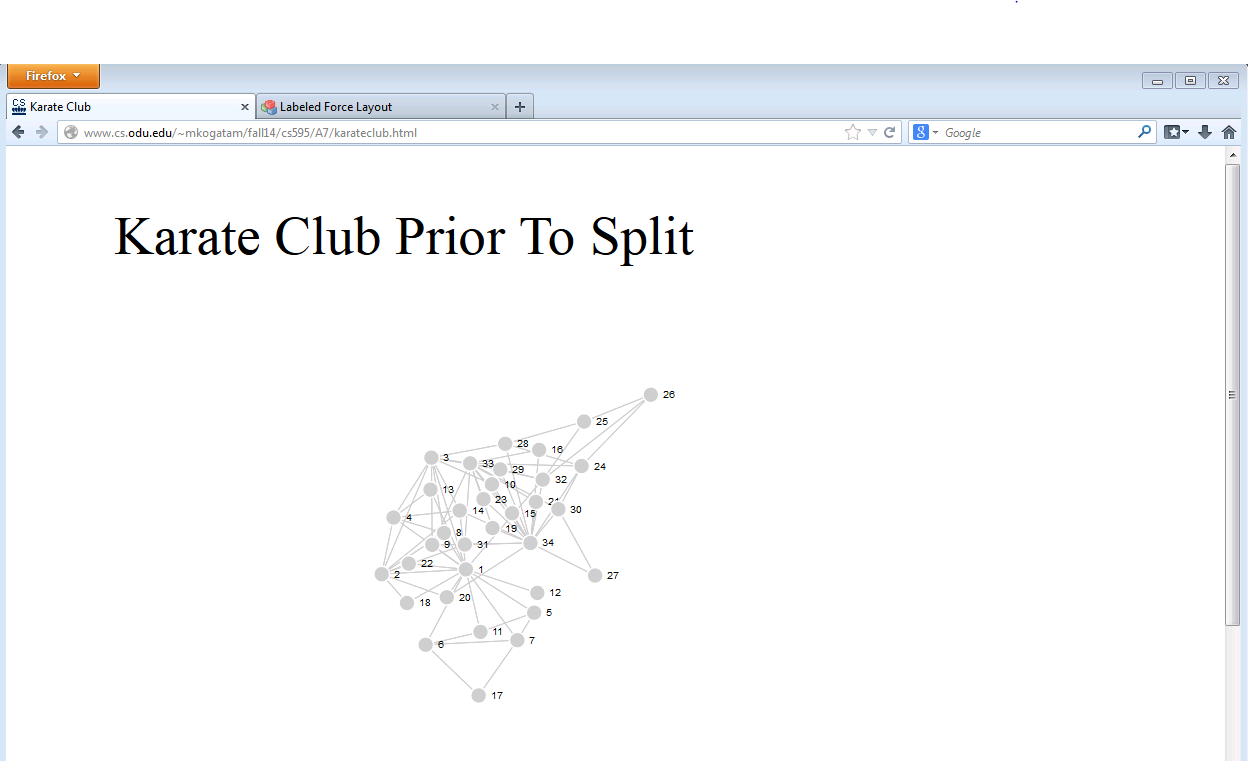
\includegraphics[scale=0.45]{q1/karateclub-beforesplit.PNG}
        \caption{Screenshot of Karate Club Graph Before Split Drawn in D3}
        \label{fig:kclub-beforesplit}
    \end{center}
\end{figure}

\begin{figure}[ht]    
    \begin{center}
        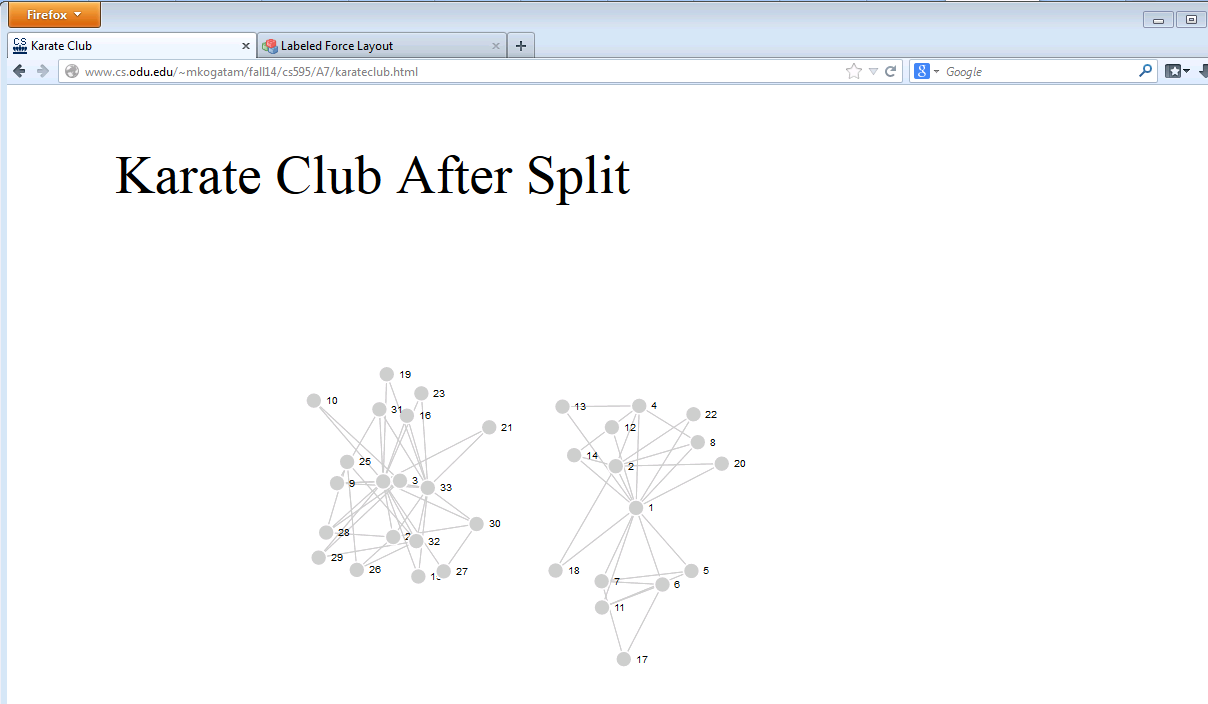
\includegraphics[scale=0.45]{q1/karateclub-aftersplit.PNG}
        \caption{Screenshot of Karate Club Graph After Split Drawn in D3}
        \label{fig:kclub-aftersplit}
    \end{center}
\end{figure}
